% LaTeX file for our ICMLA 2021 Conference submission
% Prepared as practice to familiarize myself with LaTeX
% Author: Isaiah Steinke
% Last revision: May 22, 2023

\documentclass[conference]{IEEEtran}

% Packages
\usepackage{cite}
\usepackage{amsmath,amssymb,amsfonts}
\usepackage{algorithmic}
\usepackage{graphicx}
\usepackage{textcomp}
\usepackage{xcolor}
\usepackage{hyperref} % added for URLs and internal cross-links
\usepackage{multirow} % added to customize table layout

\begin{document}

\title{Sentiment Analysis of Online Movie Reviews Using Machine Learning}

\author{\IEEEauthorblockN{1\textsuperscript{st} Given Name Surname}
\IEEEauthorblockA{\textit{dept. name of organization (of Aff.)} \\
\textit{name of organization (of Aff.)}\\
City, Country \\
email address or ORCID}
\and
\IEEEauthorblockN{2\textsuperscript{nd} Given Name Surname}
\IEEEauthorblockA{\textit{dept. name of organization (of Aff.)} \\
\textit{name of organization (of Aff.)}\\
City, Country \\
email address or ORCID}
}

\maketitle

\begin{abstract}
Many websites encourage their users to write reviews for a wide variety of products and services. In particular, movie reviews may influence the decisions of potential viewers. However, users face the arduous tasks of summarizing the information in multiple reviews and determining the useful and relevant reviews among a very large number of reviews. Therefore, we developed machine learning (ML) models to classify whether an online movie review has positive or negative sentiment. We utilized the Stanford Large Movie Review Dataset to build models using decision trees, random forests, and support vector machines (SVMs). Further, we compiled a new dataset comprising reviews from IMDb posted in 2019 and 2020 to assess whether sentiment changed owing to the coronavirus disease 2019 (COVID-19) pandemic. Our results show that the random forests and SVM models provide the best classification accuracies of 85.27\% and 86.18\%, respectively. Further, we find that movie reviews became more negative in 2020. However, statistical tests show that this change in sentiment cannot be discerned from our model predictions.
\end{abstract}

\begin{IEEEkeywords}
decision tree, machine learning (ML), natural language processing (NLP), random forests, sentiment analysis, support vector machine (SVM), reviews.
\end{IEEEkeywords}

\section{Introduction}\label{sec:Intro}
As we move more of our lives online, it becomes possible to find people's thoughts and opinions on nearly anything, from the quality of their commute to their thoughts on the most picayune political issues. One common way that people express their views online is through user reviews. These extend from assessments of mundane household items on Amazon to more commonly reviewed media such as films, music, and video games. Given the growing prevalence of online reviews, researchers have devoted a significant amount of time to determining their sentiment~\cite{ref:PangJour, ref:Sun, ref:BLiu}. The literature related to natural language processing (NLP) is extensive and outlines techniques used to process text and fit models that can determine---among other things---whether a review is positive or negative.

The importance of online reviews has increased in recent years because potential customers are increasingly using them to make purchasing or viewing decisions~\cite{ref:PangJour, ref:BLiu}. However, the number of reviews for many products, movies, and TV shows is rather large, given the massive amount of data available online. As a consequence, summarizing information from multiple reviews and finding reviews that provide relevant and useful information for decision-making are tedious and formidable tasks for users. Therefore, potential movie viewers could avoid information overload using an automated method that summarizes and classifies the opinions of online movie reviews.

Since the early 2000s, the field of sentiment analysis (or opinion mining) has grown to address many of the challenges associated with determining people's opinions, emotions, and attitudes~\cite{ref:PangJour, ref:Sun, ref:BLiu}. This field has seen explosive growth in the past two decades mainly because of the increased use of social media, the aggregation of reviews on many websites, the prevalence of blogs, and the increased use and development of machine learning (ML) techniques for NLP. Further, the opinions of consumers have had great value in business, politics, marketing, and public relations~\cite{ref:BLiu}, as determining the opinions of consumers can potentially result in large monetary savings.

In this study, we utilize sentiment analysis to determine a user's sentiment towards a movie using only that user's review (i.e., document-level analysis). Established in 1990, the Internet Movie Database (IMDb)~\cite{ref:IMDb} remains a reliable reference for film aficionados, and popular new releases receive thousands of user reviews. Hence, we use two datasets of IMDb reviews in our analyses. The first dataset is a benchmark dataset and is used to train classification models that determine review sentiment. These models are then applied to a second dataset to analyze user reviews submitted before and during the coronavirus disease 2019 (COVID-19) pandemic. Specifically, we use these results to investigate whether there is a change in review sentiment that may be attributed to the increased stress experienced from lockdowns and the threat of COVID-19 infection.

\section{Related Work}\label{sec:RelatedWork}
Sentiment analysis is currently a very active area of research, especially given the prevalence of vast amounts of data on the Internet that can be mined for sentiment. Sun \emph{et al.}~\cite{ref:Sun} review a variety of NLP techniques for this purpose. They report that the most popular techniques are na\"{i}ve Bayes classifiers, support vector machines (SVMs), latent Dirichlet allocation (LDA), and a variety of neural networks. Further, they discuss the notable preprocessing techniques used for NLP, which include tokenization, word segmentation, part-of-speech (POS) tagging, and parsing. In addition, they review toolkits that are currently available, supervised and unsupervised techniques, and opinion mining at various levels, e.g., document- and sentence-level opinion mining.

Many of the challenges associated with sentiment analysis have been outlined in the surveys in \cite{ref:PangJour} and \cite{ref:BLiu}. In particular, a review may contain both positive and negative sentiments, but the review itself may be either positive, negative, or neutral. Further, a review may contain many words associated with positive sentiment, but the review may be, for example, negative overall. An early study by Pang \emph{et al.}~\cite{ref:PangConf} showed that the use of a human-derived list of keywords to determine sentiment at the document level performed worse than a list of keywords chosen with simple statistics. Moreover, some of the keywords chosen with simple statistics would likely not be chosen by a human to determine sentiment.

Hirschberg and Manning \cite{ref:Hirschberg} review the latest advances in NLP, focusing on advanced topics such as machine translation, spoken dialogue systems, conversational agents, and machine reading. They also discuss the mining of data on social media, which is a rich area for sentiment analysis. Nadkarni \emph{et al.}~\cite{ref:Nadkarni} present an introduction to NLP as it pertains to the medical field, particularly issues that are related to clinical text. They also provide a brief overview of the techniques preferred for medical NLP, which include SVMs, hidden Markov models (HMMs), and conditional random fields (CRFs), and discuss the importance of N-grams.

Hu and Liu~\cite{ref:Hu} present a set of techniques to mine and summarize consumer reviews of products. They demonstrate that their techniques are able to provide useful feature-based summaries of products sold online. The summarization of movie reviews has also been studied using RapidMiner~\cite{ref:Alsaqer} and in mobile environments~\cite{ref:CLiu}.

Many researchers have used NLP techniques to analyze the sentiment of movie reviews. Pouransari and Ghili~\cite{ref:Pouransari} classified two datasets---one with binary class labels and the other with multiple classes---using random forests, SVMs, logistic regression, and recursive neural tensor networks (RNTNs). They propose a new type of RNTN called a low-rank RNTN, which is able to reduce computational costs compared to the standard RNTN while retaining a similar accuracy. Govindarajan~\cite{ref:Govindarajan} utilized na\"{i}ve Bayes and genetic algorithm (GA) classifiers to classify movie reviews, achieving an accuracy of just over \(91\%\) with these two classifiers separately. Moreover, they were able to increase the accuracy to \(93.80\%\) using a hybrid na\"{i}ve Bayes/GA classifier. Khan \emph{et al.}~\cite{ref:Khan} presented a method for the classification and summarization of movie reviews. To improve classification accuracy, their method employs unigrams, bigrams, and trigrams. They were able to achieve high accuracies (\(\sim\)\(90\%\)) on three different datasets using a na\"{i}ve Bayes classifier with their proposed method.

Sahu and Ahuja~\cite{ref:Sahu} utilize feature extraction and ranking to train classifiers based on decision trees, random forests, \(k\) nearest neighbors (KNN), na\"{i}ve Bayes, and bagging. They achieved accuracies as high as \(88.95\%\) with random forests. Kumar \emph{et al.}~\cite{ref:Kumar} use a hybrid feature extraction method to determine the sentiment of IMDb movie reviews. They employed SVM, na\"{i}ve Bayes, KNN, and maximum entropy classifiers, realizing an accuracy as high as \(83.9\%\) with the maximum entropy classifier.

Many of the techniques used in previous studies require high-performance computational resources, e.g., neural networks. Hence, given our available computational resources, we chose to build models using decision trees, random forests, and SVMs. These techniques were chosen because they are well-established powerful ML techniques with robust performance and prior use by other researchers in the NLP domain. Further, these techniques do not require high-performance computational resources and have achieved some of the best classification accuracies according to literature results.

\section{Data}\label{sec:Data}

\subsection{Stanford Large Movie Review Dataset}\label{sec:Stanford}
To build suitable models for the classification of movie reviews, we used the benchmark dataset, ``Large Movie Review Dataset,'' compiled by researchers at Stanford~\cite{ref:MaasDataset, ref:MaasPaper} (we will refer to this dataset as the ``Stanford dataset'' hereafter). This dataset contains 50,000 reviews from IMDb, which are evenly split into training and test sets, each with 25,000 reviews. Each review is stored in a separate plain text file. In addition, each of the test and training sets are evenly balanced to contain 12,500 positive and negative reviews. Positive reviews are defined as reviews with IMDb ratings of 7 or higher, while negative reviews have ratings of 4 or lower. Neutral reviews were excluded from this dataset. Moreover, the number of reviews was limited to no more than 30 per movie since reviews for the same movie tend to have correlated ratings. Finally, the training and test sets comprise a disjoint set of movies, which avoids the potential for performance gains by ``memorizing'' movie-specific terms.

\subsection{IMDb Dataset}\label{sec:IMDb}
To test for potential changes in sentiment amid the COVID-19 pandemic, we assembled our own dataset of 2,498 IMDb reviews for films released in 2019 and 2020. First, we determined the top 100 films released each year according to popularity by the number of ratings that a film received. We further narrowed this list by removing films released in January through March in 2020, as the effects of COVID-19 were not fully prevalent throughout the U.S. until mid-March. We also removed films that did not receive a U.S. release to mitigate the potential problem of foreign language reviews. After these steps, we selected the top 50 films according to the number of ratings for each year.

Second, we scraped the first page of reviews (25 reviews per page, except for two cases) and the rating assigned by the user; for a review with no rating provided by the user, the rating was input as NA. The final dataset includes 1,249 reviews from 2019 and 1,249 reviews from 2020 with data related to the film's alphanumeric IMDb code, title, date, average rating, number of ratings, year, and the individual user review and rating.

\section{Analysis Methods}\label{sec:Methods}
\subsection{Preprocessing}\label{sec:Preprocessing}

\begin{figure}[tbp]
    \centerline{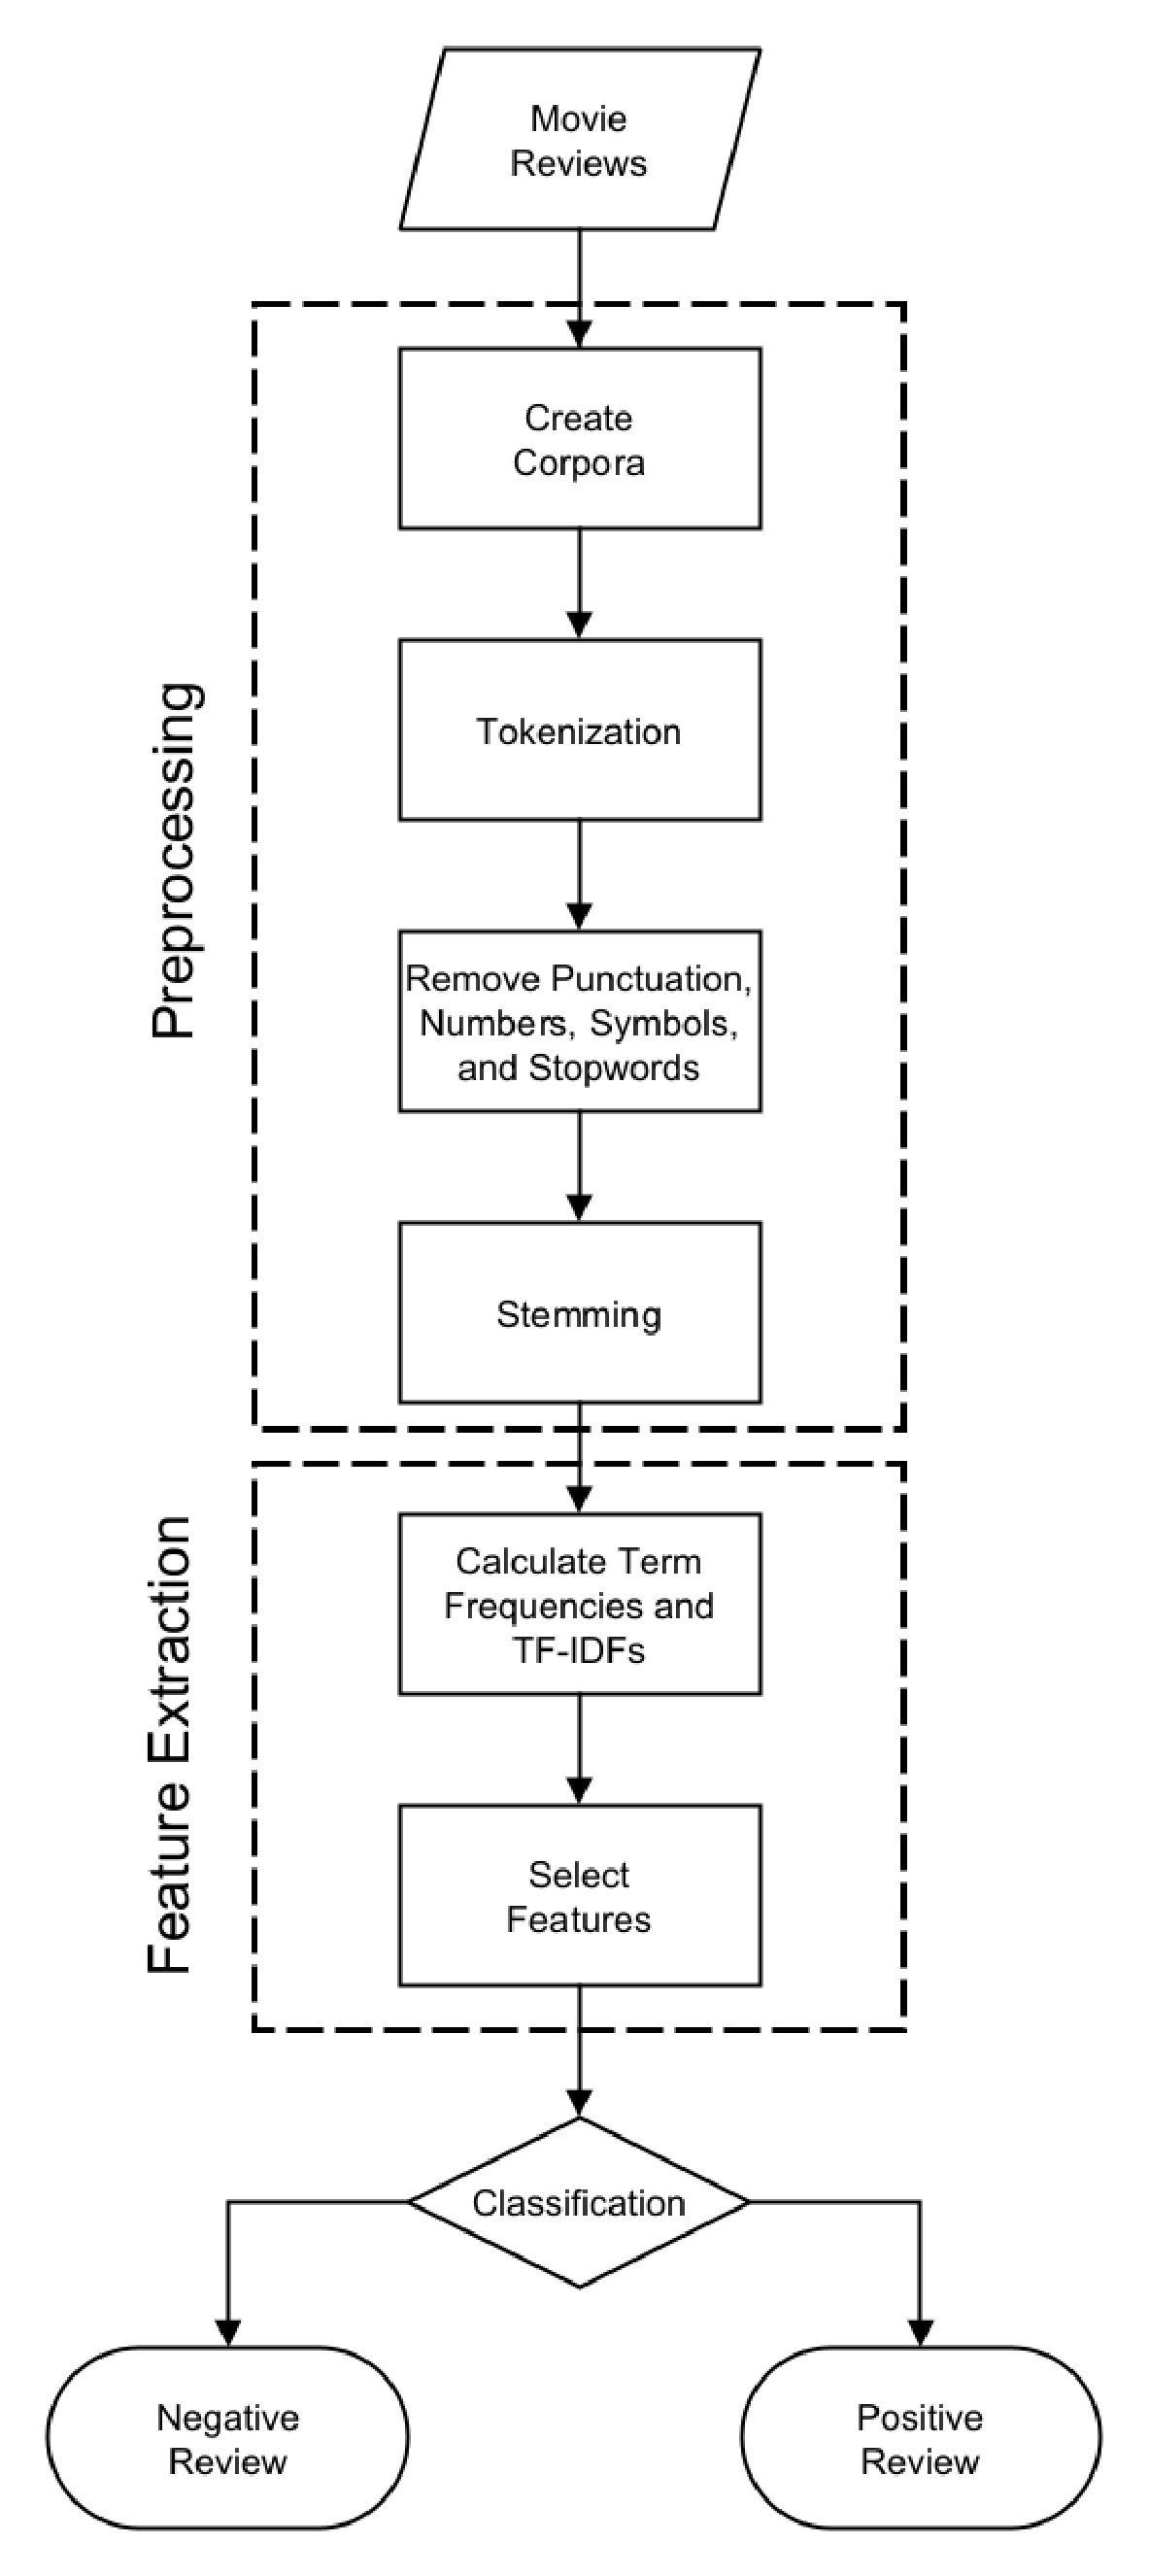
\includegraphics[width=3in]{figures/Pipeline.eps}}
    \caption{Flowchart of our model process.}
    \label{fig:Pipeline}
\end{figure}

% Note that changing the location of the code for figures can change the location of a figure in the output. For example, I've the code above was moved to before the paragraph where the figure is first cited. In the output PDF, the figure is located in the left column instead of the right column when the code is placed after the first paragraph in which the figure is first cited.

Fig.~\ref{fig:Pipeline} shows the overall flow of our model process. The raw textual reviews require preprocessing before they can be input into classification models. We utilized the \verb|quanteda| (v.~2.1.2) package in R (v.~4.0.3) to carry out much of this preprocessing. After constructing corpora of reviews, each text review was tokenized, and punctuation, symbols, and numbers were removed. In addition, we removed common English-language stopwords such as ``a,'' ``the,'' ``of,'' and other frequently occurring words that offer little information related to sentiment. We then converted all words to lower case and reduced them to word stems (e.g., ``worst'' and ``worse'' both reduce to the ``wors'' stem). The use of stemming reduces the total number of features, which is helpful for reducing the computational costs associated with model building.

After calculating the term frequencies for each word stem in each review in the corpora, we calculated the term frequency--inverse document frequency (TF-IDF) for each word stem. The TF-IDF weights the term frequency for a word stem by the inverse of its document frequency in a corpus. Thus, a word stem with a high term frequency that appears in many reviews will have a lower TF-IDF, as it will not be of much use in distinguishing sentiment since it appears in many reviews.

Initially, we built a simple decision tree model with the top 2,500 features having the highest TF-IDFs. The resulting decision tree was primarily built from nine features, all of which were ranked in the top 250 features according to TF-IDF. As more complex models require considerable computation times, we reduced the dataset to use the top 1,000 features with the highest TF-IDFs. Thus, our full training set contained 25,000 reviews with 1,000 features as the input to our models.

The IMDb dataset was preprocessed in the same way as the Stanford dataset so that it used the same 1,000 features/word stems. We also created two versions of the IMDb data. One, which we will refer to as the ``unfiltered'' version, includes all 2,498 observations/reviews. This means that reviews with ratings of 5 or 6 and those labeled NA were retained. The other, which we will refer to as the ``filtered'' version, was processed in a similar manner as the Stanford dataset. That is, reviews with ratings of 5, 6, or NA were removed. This reduced the number of reviews to 1,063 for the 2019 films and 1,048 for the 2020 films.

In addition to the 1,000 features, we also explored the use of an additional feature: the length of (or total number of words in) a review. However, after comparing histograms of this feature for the negative and positive reviews in both the training and test sets of the Stanford dataset, we found that the central values and distributions were quite similar. Hence, we did not incorporate this feature since it did not appear that the lengths of reviews would be an effective discriminator of negative and positive reviews.

\subsection{Exploratory Analysis of the IMDb Dataset}\label{sec:EDA_IMDb}
In sentiment analysis, visualization of the data is often beneficial for understanding the results. After preprocessing all of the textual data in the IMDb dataset, a list of the top 1,000 features according to TF-IDF was reclassified for visualization. By cross-referencing the term frequencies within positive, negative, and neutral reviews, each of the top 1,000 words was assigned a corresponding class. We then used the R package \verb|wordcloud| (v.~2.6) to visualize the 200 most dominant features, as shown in Fig.~\ref{fig:WordCloud}. At a glance, we see that common word stems such as ``charact'' and ``feel'' fall into the neutral category and have little use in determining the sentiment of a review. Word stems such as ``bad,'' ``noth,'' and ``dont'' dominate the negative class, and ``good,'' ``great,'' and ``watch'' stand out for the positive class.

\begin{figure}[tbp]
    \centerline{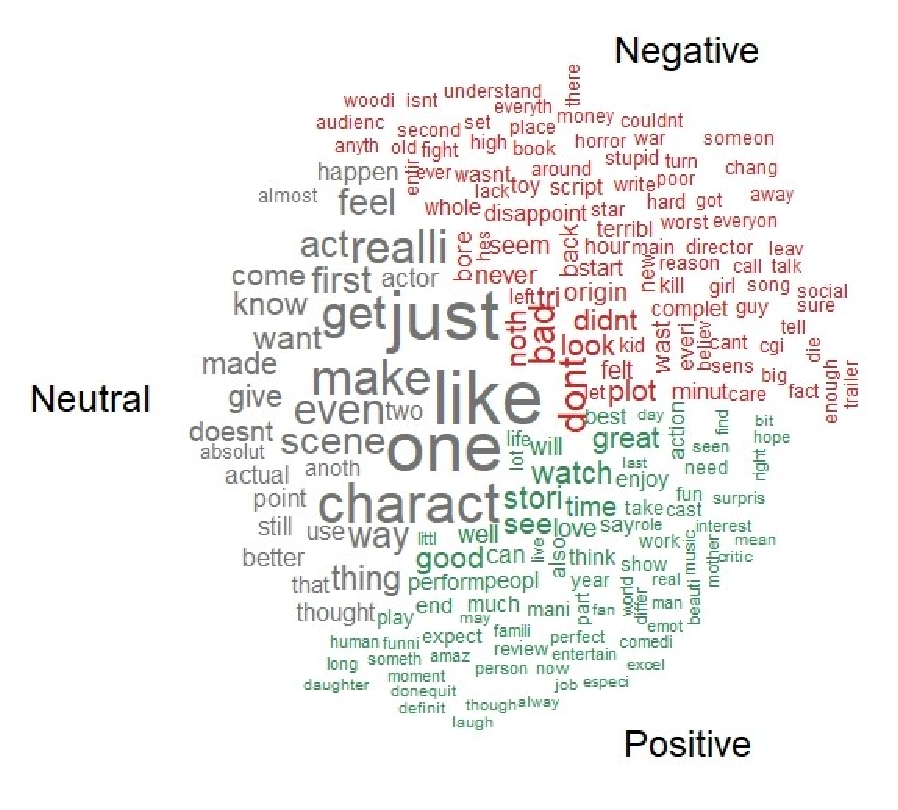
\includegraphics[width=3in]{figures/WordCloud.eps}}
    \caption{Word cloud of the 200 most prevalent terms in the IMDb dataset categorized as negative, neutral, and positive.}
    \label{fig:WordCloud}
\end{figure}

Fig.~\ref{fig:Histograms}(a) and \ref{fig:Histograms}(b) show histograms of the ratings of the reviews in the IMDb dataset for movies released in 2019 and 2020, respectively. Note that movies with no rating (i.e., ``NA'') are not accounted for in these histograms. This is a rather small number of ratings: 29 and 28 for 2019 and 2020, respectively. For both years, the numbers of reviews at the extreme ends of the scale, i.e., ratings of 1 and 10, tend to be the highest. Moreover, there is a notable decrease in the number of reviews with a rating of 10 from 2019 to 2020 (with a nearly corresponding increase in movies with a rating of 1)

\begin{figure}[tbp]
    \centerline{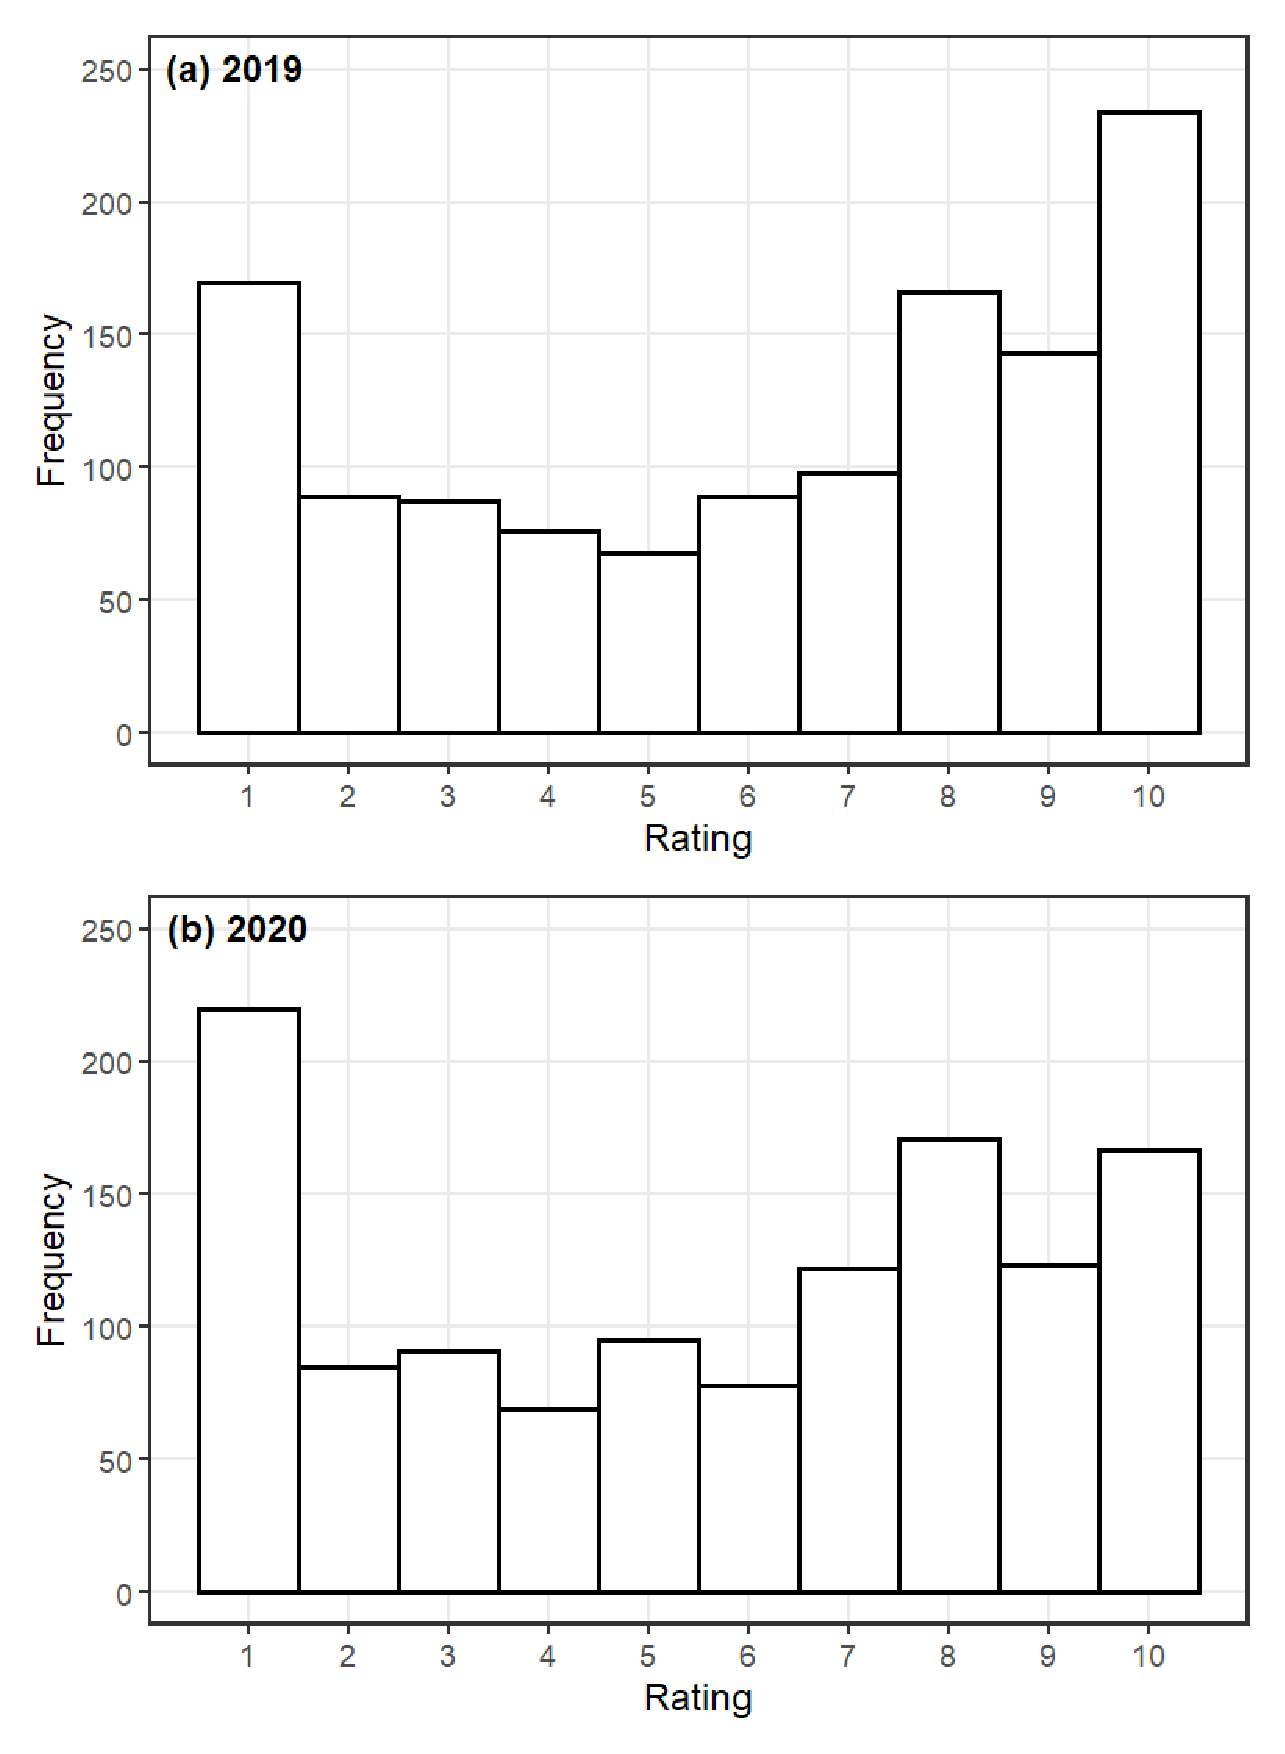
\includegraphics[width=3in]{figures/IMDbHist.eps}}
    \caption{Histograms of the ratings of reviews in the IMDb dataset for movies released in (a) 2019 and (b) 2020.}
    \label{fig:Histograms}
\end{figure}

\subsection{Modeling}\label{sec:Modeling}
All modeling and analyses were carried out in R (v.~4.0.3) on a computer equipped with an AMD Ryzen 7 3800X processor (operating at 3.9/4.5~GHz base/boost clocks) and 32~GB of RAM. We built models using decision trees, random forests, and SVMs, which were respectively implemented using the \verb|rpart| (v.~4.1-15), \verb|ranger| (v.~0.12.1), and \verb|e1071| (v.~1.7-6) packages in R. In particular, the \verb|ranger| package allows trees to be built in parallel, which provides a considerable reduction in runtime when building the models.

Since the size of the training set is sufficiently large (25,000 observations), the full training set was split at a ratio of 80:20 into training and validation sets. Given the runtimes for building the random forests and SVM models and our time constraints, we decided against the use of cross-validation (CV) and instead used a single validation set. Models were built using the reduced training set containing 20,000 observations. The validation set containing 5,000 observations was used to tune the hyperparameters of the random forests and SVM models. For the decision tree model, no parameters needed to be tuned.

For the Stanford dataset, we have a binary classification problem, i.e., a review to be classified as either positive or negative. After building a model on the reduced training set, we tested its performance on the validation set by comparing the class predicted by the model to the actual class. These results are typically summarized with a confusion matrix, from which the numbers of true positives \(n_\mathrm{TP}\), true negatives \(n_\mathrm{TN}\), false positives \(n_\mathrm{FP}\), and false negatives \(n_\mathrm{FN}\) are obtained. Using these quantities, we assessed the performance of our models using the accuracy \(A\), precision \(P\), recall \(R\), and F1-score (hereafter denoted by \(F_1\)), which are expressed as

% Note: The notation for some of the variables has changed from the original Word document submitted to ICMLA. I have changed the notation to use more standard mathematical conventions.

\begin{equation}
    A=\frac{n_\mathrm{TP} + n_\mathrm{TN}}{n_\mathrm{TP} + n_\mathrm{TN} + n_\mathrm{FP} + n_\mathrm{FN}},
    \label{eq:Acc}
\end{equation}

\begin{equation}
    P=\frac{n_\mathrm{TP}}{n_\mathrm{TP} + n_\mathrm{FP}},
    \label{eq:Pre}
\end{equation}

\begin{equation}
    R=\frac{n_\mathrm{TP}}{n_\mathrm{TP} + n_\mathrm{FN}},
    \label{eq:Rec}
\end{equation}

\begin{equation}
    F_1=\frac{2PR}{P + R}.
    \label{eq:F1}
\end{equation}

For the random forests model, we tuned the number of trees, \(n_{trees}\), and the number of predictors sampled at each split, \(n_{preds}\), using the training and validation sets with a grid search. The number of trees was varied from 100 to 1000, and the number of predictors was varied from 5 to 200. The hyperparameter values that provided the best overall values of \(A\), \(P\), \(R\), and \(F_1\) on the validation set were \(n_{trees} = 1,000\) and \(n_{preds} = 5\). These values were then used for the random forests model in subsequent analyses. We additionally tuned the minimum number of observations in a node but found that this parameter did not substantially increase \(A\); thus, we used the default value.

For the SVM models, we tuned the hyperparameters for two different kernels: linear and radial. For the linear kernel, we only tuned one parameter, the cost \(C\), which controls the bias--variance tradeoff \cite{ref:ISLR}, over the range of 0.01--1000. For the radial kernel, the hyperparameter \(\gamma\) was also tuned in addition to \(C\). For this kernel, \(C\) was varied in the range of 1--100, and \(\gamma\) ranged from 0.5 to 5. We found that the radial kernel with \(C = 10\) and \(\gamma = 1\) resulted in the best overall values for \(A\), \(P\), \(R\), and \(F_1\) on the validation set. Again, these values were then used for the SVM model in subsequent analyses. Finally, we also attempted to build SVM models with a polynomial kernel. For the few sets of hyperparameters we tried with this kernel, we obtained poor classification performance on the validation set. For all cases, the models always predicted that a review would be negative, resulting in a low value of \(A\) of 0.5. Hence, we did not further tune models with this kernel.

\section{Results}\label{sec:Results}
\subsection{Performance of the Models on the Test Set of the Stanford Dataset}\label{sec:Perf_Stanford}
Table~\ref{tab:Perf} summarizes the performance metrics in \eqref{eq:Acc}--\eqref{eq:F1} for the decision tree, random forests, and SVM models for the test set of the Stanford dataset. The random forests and SVM models use the best parameters discussed in Section~\ref{sec:Modeling}. We see that the decision tree achieves \(A = 73.78\%\). However, we can greatly increase \(A\) to \(85.27\%\) and \(86.18\%\) with the random forests and SVM models, respectively. Moreover, the random forests and SVM models provide large increases in \(P\), \(R\), and \(F_1\) relative to the decision tree model. Overall, the SVM model has the best overall performance, even though \(P\) is slightly higher for random forests.

\begin{table}[tbp]
    \caption{Performance Metrics for the Models on the Test Set of the Stanford Dataset}
    \begin{center}
    \begin{tabular}{c|cccc}
    \hline
    \textbf{Model} & \(A\) & \(P\) & \(R\) & \(F_1\) \\
    \hline
    Decision Tree & \(73.78\%\) & \(71.40\%\) & \(79.34\%\) & \(75.16\%\) \\
    Random Forests & \(85.27\%\) & \(84.93\%\) & \(85.77\%\) & \(85.34\%\) \\
    SVM & \(86.18\%\) & \(84.62\%\) & \(88.45\%\) & \(86.49\%\) \\
    \hline
    \end{tabular}
    \label{tab:Perf}
    \end{center}
\end{table}

\subsection{Variable Importance for the Tree-Based Models}\label{sec:VarImp}
For the decision tree model, we noted the variables used in the construction of the tree and their importance. In addition, we looked at the variable importance of the features in the random forests model using the best parameters in Section~\ref{sec:Modeling}. Fig.~\ref{fig:VarImp}(a) and \ref{fig:VarImp}(b) show plots of the 10 most important variables for the decision tree and random forests models, respectively.

\begin{figure}[tbp]
    \centerline{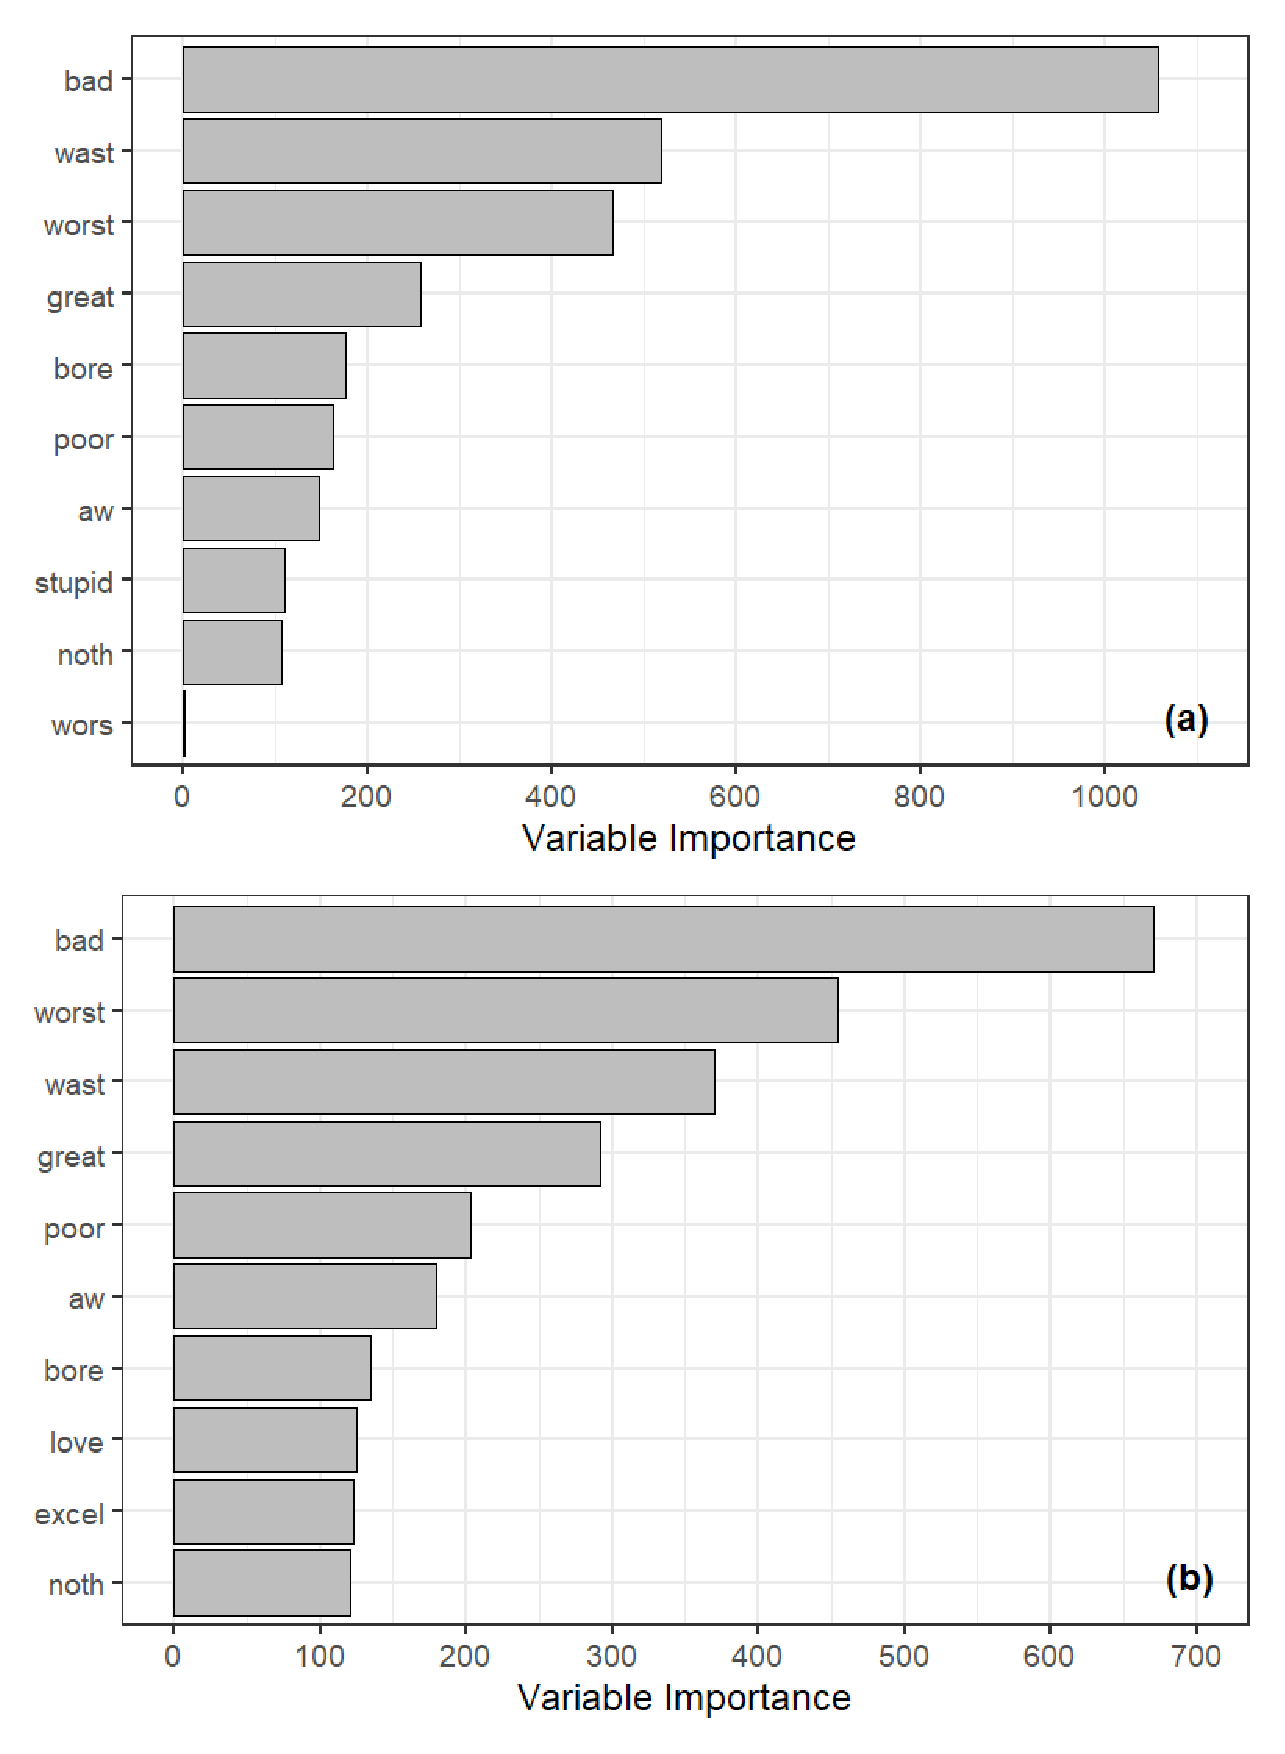
\includegraphics[width=3in]{figures/VarImp.eps}}
    \caption{Plots of the 10 most important variables for the (a) decision tree and (b) random forests models.}
    \label{fig:VarImp}
\end{figure}

Both of the decision tree and random forests models found ``bad'' to be the feature of highest importance. The same eight words appear in the top 10 features of both methods with varying degrees of importance. Further, the majority of these word stems fall into the negative category in the word cloud analysis (e.g., ``bad,'' ``bore,'' and ``wast'') with some positive word stems (e.g., ``great'' and ``excel''). Notably, these terms make intuitive sense for distinguishing negative and positive movie reviews.

\subsection{IMDb Dataset}\label{sec:ResultsIMDb}
We used our trained models to classify the reviews in the IMDb dataset. Table~\ref{tab:Unfilt} summarizes the percentages of movie reviews classified as negative and positive for the unfiltered IMDb dataset. The decision tree model classifies fewer reviews as negative compared to the random forests and SVM models. This is most likely related to the large difference in the performance metrics in Table~\ref{tab:Perf}, as \(A\) is much worse for the decision tree.

\begin{table}[tbp]
    \caption{Percentages of Negative and Positive Reviews Predicted by the Models for the Unfiltered IMDb Dataset}
    \begin{center}
    \begin{tabular}{c|c|cc}
    \hline
    \textbf{Year} & \textbf{Model} & \textbf{\(\%\) Negative} & \textbf{\(\%\) Positive} \\
    \hline
    \multirow[c]{3}{*}{\shortstack[c]{2019 \\ \((n = 1249)\)}} & Decision Tree & \(35.15\%\) & \(64.85\%\) \\
     & Random Forests & \(43.31\%\) & \(56.69\%\) \\
     & SVM & \(44.84\%\) & \(55.16\%\) \\
    \hline
    \multirow[c]{3}{*}{\shortstack[c]{2020 \\ \((n = 1249)\)}} & Decision Tree & \(35.23\%\) & \(64.77\%\) \\
     & Random Forests & \(46.48\%\) & \(53.72\%\) \\
     & SVM & \(48.52\%\) & \(51.48\%\) \\
    \hline
    \end{tabular}
    \label{tab:Unfilt}
    \end{center}
\end{table}

Table~\ref{tab:Filt} summarizes the percentages of movie reviews classified as negative and positive for the filtered IMDb dataset. Since this dataset has been filtered to only contain negative and positive reviews, as discussed in Section~\ref{sec:Preprocessing}, we have also tabulated the actual percentages of negative and positive reviews using the rating on IMDb for comparison. Here again, we see that the decision tree model classifies fewer reviews as negative compared to the other models. However, we see that it is the furthest away from the actual percentages than the random forests and SVM models. Surprisingly, the percentages for the random forests model are closer to the actual percentages than those for the SVM model, despite the slightly lower performance metrics for the random forests model. This may be partially attributed to the slightly higher value of \(P\) for the random forests model relative to that of the SVM model. This suggests that it might be better to tune the models to control \(n_{\mathrm{FP}}\).

\begin{table}[tbp]
    \caption{Percentages of Negative and Positive Reviews Predicted by the Models for the Filtered IMDb Dataset}
    \begin{center}
    \begin{tabular}{c|c|cc}
    \hline
    \textbf{Year} & \textbf{Model} & \textbf{\(\%\) Negative} & \textbf{\(\%\) Positive} \\
    \hline
    \multirow[c]{4}{*}{\shortstack[c]{2019 \\ \((n = 1063)\)}} & Decision Tree & \(33.68\%\) & \(66.32\%\) \\
     & Random Forests & \(40.73\%\) & \(59.27\%\) \\
     & SVM & \(42.80\%\) & \(57.20\%\) \\
     & Actual & \(39.70\%\) & \(60.30\%\) \\
    \hline
    \multirow[c]{4}{*}{\shortstack[c]{2020 \\ \((n = 1048)\)}} & Decision Tree & \(33.87\%\) & \(66.13\%\) \\
     & Random Forests & \(44.08\%\) & \(55.92\%\) \\
     & SVM & \(46.18\%\) & \(53.82\%\) \\
     & Actual & \(44.37\%\) & \(55.63\%\) \\
    \hline
    \end{tabular}
    \label{tab:Filt}
    \end{center}
\end{table}

The results in Tables~\ref{tab:Unfilt} and \ref{tab:Filt} show that the percentage of negative reviews increases from 2019 to 2020 for all models and for the actual data. This is also observed in the histograms in Fig.~\ref{fig:Histograms}. To ascertain whether these results were real, we conducted a chi-squared test of homogeneity~\cite{ref:Ott1}. For the unfiltered IMDb data, we found that both of the random forests (\(p = 0.1475\)) and SVM (\(p = 0.0711\)) models did not show a statistically significant difference in the distribution of percentages at a level of significance, \(\alpha\), of 0.05. For the filtered IMDb data, the conclusion was the same for random forests (\(p = 0.1302\)) and SVM (\(p = 0.1289\)). However, if we carry out this test with the actual data (\(p = 0.0332\)), we find that there is a statistically significant difference. Thus, even though there is statistical evidence that there is a change in sentiment from 2019 to 2020 in the actual data, our models do not appear to be sufficiently performant to indicate this difference. This could be an important consideration if we wish to use our models to ascertain changes in sentiment over time, especially if we have unsupervised data, i.e., reviews with no ratings.

We also carried out additional statistical tests of the difference between two population proportions~\cite{ref:Ott2} to confirm these results. Here, we only chose to test the SVM model, which has the highest overall performance. Again, there is no statistical evidence (at \(\alpha = 0.05\)) that there is a difference between population proportions for the unfiltered (\(p = 0.0651\)) and filtered (\(p = 0.1180\)) IMDb sets. However, the actual data do indicate that there is statistical evidence of a difference in proportions (\(p = 0.0298\)), as before.

\section{Discussion and Conclusion}\label{sec:Conclusion}
We have developed models using decision tree, random forests, and SVM ML techniques to classify the sentiment of movie reviews. Our models were trained and built on the Stanford dataset, which is a benchmark dataset in the literature. In addition, we constructed a new dataset consisting of movie reviews from IMDb posted in 2019 and 2020. Using the Stanford dataset, we find that the SVM model provides the best overall performance, with \(A = 86.18\%\), \(P = 84.62\%\), \(R = 88.45\%\), and \(F_1 = 86.49\%\). The random forests model also provides good performance that is slightly worse than the SVM model. The variables that are important for the tree-based models are quite similar, and they tend to utilize words that would be useful in distinguishing negative and positive reviews.

For our IMDb dataset, we find that the random forests and SVM models tend to classify more reviews as negative compared to the decision tree model. Moreover, the random forests model more closely replicates the actual percentages of negative and positive reviews in our filtered IMDb set. However, the models are not able to provide statistical evidence of a change in sentiment from 2019 to 2020. The actual percentages of negative and positive reviews indicate that there is a change in sentiment; that is, issues related to the COVID-19 pandemic may have resulted in an increase in negative reviews. Further time-series analyses may be needed to tell if the increase in negative reviews can be solely attributed to the COVID-19 pandemic. Our analysis does not consider whether this increase was a result of increased negative attitudes elicited by pandemic stressors; studios' decisions to postpone high-profile releases such as Black Widow, Dune, F9, and No Time to Die; and other factors that we did not consider.

There is considerable scope for improvement in the performance of our models. During preprocessing, we reduced the number of features to the top 1,000 features according to the TF-IDF. This was done solely to keep the computational times of our models to a reasonable level within our time constraints. It is possible that we may realize additional improvements by increasing the number of features. Further, we did not utilize any feature-reduction techniques, e.g., singular value decomposition (SVD), which may also be employed to increase performance. Although the term frequencies were calculated, we did not build models using them, as longer reviews that repeat a unique term could bias the term frequencies. However, it is possible that models built with the term frequencies could provide better results, especially if we remove terms that appear in both negative and positive reviews at high frequencies. Our time constraints also reduced the number of hyperparameter combinations that we could test and prevented us from employing CV. Additional hyperparameter tuning and CV could increase the performance of our models, although we expect that this is likely to be limited to a few percentage points.

Our models were simple bag-of-words (BoW) models that only used unigrams. As shown by Khan \emph{et al.}~\cite{ref:Khan}, we may improve classification performance by including more complex two- and three-word phrases (i.e., bigrams and trigrams, respectively). By using bigrams, a phrase such as ``no good,'' which has a negative connotation, would be used as a bigram instead of the unigrams ``no'' and ``good,'' which have negative and positive connotations, respectively.

Finally, we were only able to test a small number of ML techniques. According to the literature review in Section II, other techniques can be used to achieve quite high classification accuracies of more than \(90\%\), e.g., na\"{i}ve Bayes classifiers, GA classifiers, and many types of neural networks. Hence, additional techniques could be employed in future work to increase classification performance.

% References

% BiBTeX references
\bibliographystyle{IEEEtran}
\IEEEtriggeratref{7} % inserted to roughly equalize columns on last page
\bibliography{bibtex/refs}

% Manually entered references
% \begin{thebibliography}{99}
% \bibitem{ref:PangJour} B.~Pang and L.~Lee, ``Opinion mining and sentiment analysis,'' \textit{Found. Trends Inform. Retrieval}, vol.~2, no.~1--2, pp.~1--135, 2008.
% \bibitem{ref:Sun} S.~Sun, C.~Luo, and J.~Chen, ``A review of natural language processing techniques for opinion mining systems,'' \textit{Inform. Fusion}, vol.~36, pp.~10--25, 2017.
% \bibitem{ref:BLiu} B.~Liu, ``Sentiment analysis and opinion mining,'' in Synthesis Lectures on Human Language Technologies, G.~Hirst, Ed. San Rafael, CA, USA: Morgan \& Claypool, 2012, pp.~1--167.
% \bibitem{ref:IMDb} ``Internet Movie Database (IMDb),'' \url{http://www.imdb.com} (accessed Apr. 23, 2021).
% \bibitem{ref:PangConf} B.~Pang, L.~Lee, and S.~Vaithyanathan, ``Thumbs up? Sentiment classification using machine learning techniques,'' in \textit{Proc. Conf. Empirical Methods in Natural Language Processing (EMNLP)}, 2002, pp.~79--86.
% \bibitem{ref:Hirschberg} J.~Hirschberg and C.~D.~Manning, ``Advances in natural language processing,'' \textit{Science}, vol.~349, no.~6245, pp.~261--266, Jul. 2015.
% \newpage % inserted to roughly equalize columns on last page, as recommended by IEEE; move as needed
% \bibitem{ref:Nadkarni} P.~M.~Nadkarni, L.~Ohno-Machado, and W.~W.~Chapman, ``Natural language processing: An introduction,'' \textit{J. Am. Med. Inform. Assoc.}, vol.~18, pp.~544--551, 2011.
% \bibitem{ref:Hu} M.~Hu and B.~Liu, ``Mining and summarizing customer reviews,'' in \textit{Proc. Tenth ACM SIGKDD Int. Conf. Knowledge Discovery and Data Mining}, Aug. 2004, pp.~168--177.
% \bibitem{ref:Alsaqer} A.~F.~Alsaqer and S.~Sasi, ``Movie review summarization and sentiment analysis using RapidMiner,'' in \textit{2017 Int. Conf. Networks \& Advances in Computational Technologies (NetACT)}, pp.~329--335.
% \bibitem{ref:CLiu} C.-L.~Liu, W.-H.~Hsaio, C.-H.~Lee, G.-C.~Lu, and E.~Jou, ``Movie rating and review summarization in mobile environment,'' \textit{IEEE Trans. Syst., Man, Cybern. Syst. C, Appl. Reviews}, vol.~42, no.~3, pp.~397--407, May 2012.
% \bibitem{ref:Pouransari} H.~Pouransari and S.~Ghili, ``Deep learning for sentiment analysis of movie reviews,'' 2015. [Online]. Available: \url{https://cs224d.stanford.edu/reports/PouransariHadi.pdf}.
% \bibitem{ref:Govindarajan} M.~Govindarajan, ``Sentiment analysis of movie reviews using hybrid method of naive Bayes and genetic algorithm,'' \textit{Int. J. Adv. Comput. Res.}, vol.~3, no.~4, pp.~139--145, Dec. 2013.
% \bibitem{ref:Khan} A.~Khan \textit{et al.}, ``Summarizing online movie reviews: A machine learning approach to big data analytics,'' \textit{Sci. Program.}, vol.~2020, Art.~no.~5812715, Aug. 2020.
% \bibitem{ref:Sahu} T.~P.~Sahu and S.~Ahuja, ``Sentiment analysis of movie reviews: A study on feature selection \& classification algorithms,'' in \textit{2016 Int. Conf. Microelectronics, Computing and Communications (MicroCom)}.
% \bibitem{ref:Kumar} H.~M.~Keerthi Kumar, B.~S.~Harish, and H.~K.~Darshan, ``Sentiment analysis on IMDb movie reviews using hybrid feature extraction method,'' \textit{Int. J. Interact. Multimedia Artif. Intell.}, vol.~5, no.~5, pp.~109--114, 2018.
% \bibitem{ref:MaasDataset} A.~Maas, 2011, ``Large Movie Review Dataset,'' Stanford AI Lab. [Online]. Available: \url{http://ai.stanford.edu/~amaas/data/sentiment/}.
% \bibitem{ref:MaasPaper} A.~L.~Maas, R.~E.~Daly, P.~T.~Pham, D.~Huang, A.~Y.~Ng, and C.~Potts, ``Learning word vectors for sentiment analysis,'' in \textit{49th Annu. Meeting Association for Computational Linguistics (ACL 2011)}.
% \bibitem{ref:ISLR} G.~James, D.~Witten, T.~Hastie, and R.~Tibshirani, \textit{An Introduction to Statistical Learning with Applications in R}, 1st ed. New York, NY, USA: Springer, 2013, ch.~9.
% \bibitem{ref:Ott1} R.~L.~Ott and M.~Longnecker, \textit{An Introduction to Statistical Methods \& Data Analysis}, 7th ed. Boston, MA, USA: Cengage Learning, 2016, sec.~10.5.
% \bibitem{ref:Ott2} R.~L.~Ott and M.~Longnecker, An Introduction to Statistical Methods \& Data Analysis, 7th ed. Boston, MA, USA: Cengage Learning, 2016, sec.~10.3.
% \end{thebibliography}

\end{document}
